\chapter{Results}\label{ch:results}

Please note: this chapter is written as a demonstrator section for expediency. The original plan was to draw out from the interviews mentions pertaining to each factor in the ISM framework. However, this is proving to be a huge undertaking. Instead, I propose to only work with a few of the factors that are relevant to scientists' roles. For instance, these may be Values, beliefs, attitudes, (currently unfinished Section~\ref{sec:resismvalues}), Opinion leaders (currently slightly more finished Section~\ref{sec:resopinionleaders}) and Roles and identity (currently slightly more finished Section~\ref{sec:resroles}). This may be plenty if I include the discussion that ties these three elements together with published work on roles at the science policy interface. 

Where relevant below, I explain the current state of the chapter. Section~\ref{sec:resindividual}, the chapter on individual factors that influence behaviour, has not been updated from the first test run, because I have not had time - and now I wonder if most of it will be removed. Instead, I have focused more attention on Section~\ref{sec:ressocial}, the social factors that influence behaviours, because this appears to be more important to participants (based on the number of stories that mention these factors). I process the two social factors (Opinion leaders and Roles and identity) that I suggest above.

Quick summary - because there is no methods section. Within the interviews, chunks of description pertaining to the same theme were grouped into ``stories''. This was a more logical unit than sentence or participant. Each of these stories comprised multiple statements and each statement was labelled according to how it referenced one or more of 18 different factors that influence behaviour, as described in the ISM framework. I labelled on those factors that influenced the behaviour of scientists, but some of them may appear to be more to do with others (such as a policymaker requiring a \emph{skill} in CAN science, which affects how well a scientist can engage with them).

A total of 155 stories\improvement{make sure stories are explained in Chapter~\ref{ch:methods}} were identified in the interviews, excluding those pertaining to the participants' introductory statements about their field of work. Frequently, a story would contain multiple labels for the same theme. For instance, Story 45 ``frustrations as a scientist compared to those as a concerned citizen'' contained mentions of 3 different roles, as well as a description of a conflict in roles. Section~\ref{sec:resultsISM} discusses the nature of each of the ISM factors as they surface within the interviews.

\section{Drivers and barriers to CAN science-policy engagement}\label{sec:resultsISM}

\begin{figure}[!ht]
    \centering
    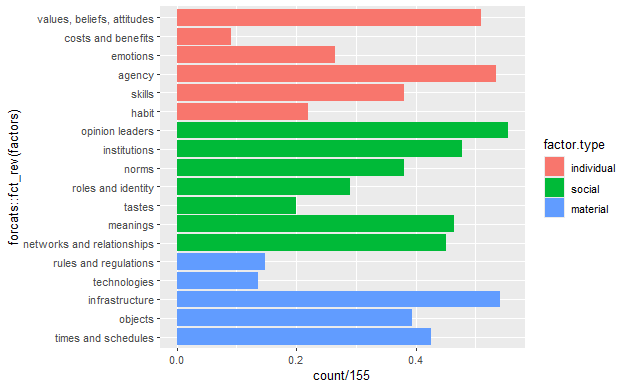
\includegraphics[width=1\linewidth]{figures/ism_count_per_story.png}
    \caption{Number of stories mentioning ISM factors}
    \label{fig:ismstorycount}
\end{figure}

The ISM framework\improvement{make sure this is explained and referenced in Chapter~\ref{ch:lit} and how I used it is described in Chapter~\ref{ch:methods}} was used to identify the behaviour factors that enable or inhibit engagement and influence at the science policy interface. Figure~\ref{fig:ismstorycount} shows the number of stories in which each factor was mentioned. Each section below describes the nature of the drivers for each of 18 behavioural factors, as identified in the interviews.


\subsection{Individual factors}\label{sec:resindividual}

Currently, this section is was the first test of the method and has not been updated. It is based on the first 6 of 18 behavioural factors and for 3 of 14 participants. It is expected (there is some evidence) that broader patterns will emerge as the analysis continues such as different `types' of scientist in regards to these different factors. The second test, in the following section~\ref{sec:ressocial}, has been applied to the interviews with all 14 participants.

\subsubsection{Values, beliefs, attitudes}\label{sec:resismvalues}
Participants stated a range of values, beliefs and attitudes that motivated them to undertake policy-relevant science and engage with policy. All indicated that their science should be \emph{useful} and, similarly, most felt that \emph{policy should be based on the best science}. One scientist has a strongly normative approach to their work, indicating that they undertook their work because they believed science should be \emph{open}, \emph{credible}, \emph{relevant} and \emph{responsible}. They also believed that they had a duty to return \emph{value for public money}. Another was more ethically-driven, indicating that they undertook their work for reasons of \emph{social justice} and that they had a \emph{duty to try}.  

\subsubsection{Costs and benefits}\label{sec:resismcab}
There was very little indication of scientists weighing up the costs and benefits of their work or that of others. One scientist balanced the value of their activity with its used for policymaking and concluded that \emph{it's worth it} - \tquote{If it's going to be useful, why wouldn't we prioritise our time to do that paper rather than something else}{p01}{}, this was linked to an acknowledgement of the costs and benefits to policymakers for whom reading all the relevant scientific literature is \emph{too much effort}. Regarding engaging at the science policy interface, another scientist felt that they were \emph{not sure its worth the effort} - \tquote{I'm not convinced that it overall is hugely impactful}{p03}{}
\subsubsection{Emotions}\label{sec:resismemotions}
Various emotions were associated with undertaking science and engaging with policy including \emph{exhaustion}, \emph{intrigue}, \emph{pleasure} and \emph{pride}. However, these were largely expressed only by one participant, with another expressing no emotions.

\subsubsection{Agency}\label{sec:resismagency}
Agency was, by far, the most commonly expressed driver or barrier to working on policy-related science and engaging with policy. There was a contrast between one scientist who frequently expressed confidence in \emph{making it happen} alongside being \emph{open to new ideas}. This contrasted with another participant who was more likely to express \emph{limits to my influence}. Most participants also noted the role of \emph{happenstance} in their ability to engage at the science policy interface. The agency of others were also noted by participants, such as the ability of NGOs in terms of \emph{making it happen} and that policymakers and stakeholders in policy (such as businesses) could be \emph{open to new ideas}.

\subsubsection{Skills}\label{sec:resismskills}
Understandably, skills were also identified as important for engaging with policy. In particular statements indicating that engagement was possible because scientists \emph{know and understand the science} and also when scientists \emph{know and understand how policy is made}. Further, participants identified that how well policymakers \emph{know and understand the science} affected engagement (if they don't know and understand, they would reach out to scientists) but also how well policy is made (if they don't know and understand the science, they can choose poor evidence for decisionmaking).

\subsubsection{Habit}\label{sec:resismhabit}
Two habits were identified within the interviews. The first, identified by all participants was the habit of \emph{scientists doing science for scientists} which tended to be less useful for policymaking. The other habit, which participants often, but not always, identified as a barrier to engagement was \emph{policy obtaining information from the same sources} rather than reaching out to scientists with more policy-challenging perspectives. This was less of a barrier in the context that scientists used this knowledge to publish their work in media deemed to be popular with policymakers.

\subsection{Social factors}\label{sec:ressocial}

This section demonstrates the second test of the method and synthesises the interviews of all 14 participants. This turned out to be a huge undertaking and I have only extracted the results for two of the 7 social factors: Opinion leaders (Section~\ref{sec:resopinionleaders}) and Roles and identity (Section~\ref{sec:resroles}). I suggest we have a deeper discussion about what would be most appropriates to continue working on - should it be to continue outlining each factor, or to focus only on those related to roles.

Figure~\ref{fig:ismstorycount} indicates that social factors are more `important' than individual or material factors.

Each section describes the results for one factor. The section includes a table which outlines each type of mention for that factor, whether the factor enabled/inhibited engagement or influence, and an example quote from the interviews. A short description of these mentions is given, followed by typical strategies applied by scientists which either exploits or counteracts the factor.

\subsubsection{Opinion leaders}\label{sec:resopinionleaders}

\begin{table}[!ht]
\footnotesize
\caption{The 7 types of mention of \emph{opinion leaders} in the interviews and example quotes for each type}\label{tab:resopinionleaders}
%\begin{tabularx}{\textwidth} {DIQ} 
\begin{tabular}{L{.08\linewidth}L{.3\linewidth}L{.1\linewidth}L{.42\linewidth}}\hline
\textbf{id} & \textbf{mention type} & \textbf{influence} & \textbf{quote} \\ \hline \hline 
ol1 & scientists' knowledge   drew interest from policymakers & enabler & \tquote{They had already decided they wanted to work with us}{p05}{}  \\[5mm]
ol2 & scientists influencing policymakers & enabler & \tquote{Informally I think they [have been] picked up and had a bit of traction}{p03}{}  \\[5mm]
ol3 & scientists influencing others & enabler & \tquote{We've been cited by both industry and NGOs on different sides of the debate, so we've probably got something right there}{p01}{} \\[5mm]
ol4 & senior scientists are more likely to be   listened to & enabler & \tquote{When it comes to something for more formal like that, they tend to go for the professors}{p03}{} \\[5mm]
ol5 & I look up to other scientists & enabler & \tquote{He's an excellent scientist, he's very inclusive and he's   incredibly motivational from a scientific perspective, very much in favour of   community building}{p04}{} \\[5mm]
ol6 & others influence policymakers & inhibitor & \tquote{Sometimes what they bring is politically convenient, and policymaking is not just about evidence is also about political convenience   or political opportunity. They provide narratives to use or discard certain evidence}{p09}{}  \\[5mm]
ol7 & policymakers have influence & neutral & \tquote{I think policy makers have the greatest leverage of   all}{p08}{} \\[5mm] \hline \hline
\textbf{id} & \textbf{strategy} &  \multicolumn{2}{L{.52\linewidth}}{\textbf{quote}} \\ \hline \hline 
ols1 & opportunities to promote my/our work & \multicolumn{2}{L{.52\linewidth}}{\tquote{If I get media requests, I think if I've got the expertise, I   should do that because it goes with the job}{p01}{}}  \\[5mm]
ols2 &  opportunities to understand the perspectives of policymakers & \multicolumn{2}{L{.52\linewidth}}{\tquote{we try and find out what their priorities are}{p12}{}} \\[5mm] \hline
\end{tabular}
%\end{tabularx}
\end{table}
\improvement{the layout of this table needs to be easier to read}

Nearly half of the stories mention individuals and groups to whom scientists and policymakers will reach out, and be influenced by - more than any other social factor. This indicates that opinion leaders are important to scientists engaging with policy. Given the criteria for inviting people to take part in this study, it is not surprising that many participants mentioned being invited by policymakers to share their knowledge (ol1). Others identified that they believed they had had some influence on policymaking (ol2) or others, such as industry and NGOs (ol3). The was specific recognition that senior scientists are more likely to have influence (ol4).  

It was also quite common to observe that there are non-science actors, such as other governments, industry, learned societies, research councils, special advisers and NGOs, who have influence in the decisions being make (ol6). Further, policymakers themselves were considered to have influence (ol7)

\paragraph{Strategies:}

In some cases, this understanding has been used to gain influence. A number of participants mentioned promoting their work through third parties such as media opportunities but also by engaging with organisations such as industry or NGOs such as charities, campaigning organisations and networks (think tanks) as a mechanism for influencing policymaking (ols1). A different approach was to make efforts to align with policymakers by taking up opportunities to listen to their perspectives (ols2).

\subsubsection{Institutions}\label{sec:resinstitutions}
\subsubsection{Norms}\label{sec:resnorms}

\subsubsection{Roles and identity}\label{sec:resroles}

\begin{table}[!ht]
\footnotesize
\caption{The \emph{roles} and \emph{identities} of scientists expressed in the interviews}\label{tab:resroles}
%\begin{tabularx}{\textwidth} {DIQ} 
\begin{tabular}{L{.08\linewidth}L{.32\linewidth}L{.5\linewidth}}\hline
\multicolumn{2}{L{.4\linewidth}}{\textbf{roles}} & \textbf{identities} \\ \hline\hline
\multicolumn{2}{L{.4\linewidth}}{academic, adviser, advocate, citizen, public servant, representative, researcher, specialist} & authoritative, candid, esteemed, experienced, expert, helpful, humble, impartial, informed, judicious, receptive, relevant, selfish \\[5mm] \hline\hline
\multicolumn{3}{L{.9\linewidth}}{\textbf{conflicts}} \\ \hline
\multicolumn{2}{L{.4\linewidth}}{citizen versus scientist} & deserving recognition \\
\multicolumn{2}{L{.4\linewidth}}{researcher versus adviser} & \\
\multicolumn{2}{L{.4\linewidth}}{adviser versus advocate} & \\[2mm] \hline\hline
\textbf{id} & \textbf{strategies} & \textbf{quote} \\ \hline
ris1 & do deeper more policy-focused research & \tquote{but a lot of scientists should actually get on and try and discover  what they think is going to be societally important stuff and it'll have policy influence through that}{p13}{} \\[5mm]
ris2 & identifying preferred role and sticking to it & \tquote{But beyond that, I consciously draw the line [between advice and advocacy]}{p09}{} \\[5mm]
ris3 & identifying the bounds of advocacy & \tquote{[I advocate] only within already societally-established parameters}{p09}{} \\[5mm]
ris4 & making a conscious pivot in role & \tquote{I have pivoted, but that's just because the demand isn't ... from ... policy makers asking me questions or trying to set a policy agenda}{p08}{} \\[5mm]
ris5 & collaborating with people in other roles & \tquote{It's a bit toe curling, which is why we also work with a charity ... who do a lot more of that}{p05}{}\\[5mm] \hline
\end{tabular}
%\end{tabularx}
\end{table}
Participants referred to theirs, or other scientists', roles or identity in about one fifth of the stories. The nature of the roles were varied. As one participant noted \tquote{scientists are a very diverse bunch}{p09}{} and the role ``scientist'' was assumed to be generic to all participants because it was the premise for the interview. Therefore, the roles played by those scientists are entered into the left column of Table~\ref{tab:resroles}, with a range of their identities in the right column. This section describes these roles and identities, the conflicts that emerge in this roles and the strategies used that relate to the conflicts.

\paragraph{Scientists' roles}
Scientists see themselves and other scientists as a \emph{researcher}, who is sometimes a \emph{specialist}. Some roles are in relation to the scientists' institution, such as \emph{academic}, \emph{representative} and \emph{public servant}, the latter referring to a scientist in a government science setting or in an academic institution with a strong awareness of its public funding (See also Section~\ref{sec:resismvalues} \emph{value for public money} and Section~\ref{sec:resinstitutions} \emph{social responsibility of public organisations}). Those working more regularly at the interface with policy, may consider themselves more as an \emph{adviser} and occasionally an \emph{advocate}. Also, a number of participants were conscious of their role as a \emph{citizen}.

\paragraph{Scientists' identities}
Identities ranged from those largely within the scientific realm concerning scientific recognition (\emph{esteemed}), ability (\emph{expert}) and duty (\emph{helpful}), to those that emerged at the interface concerning the ability to gain notice (\emph{authoritative}), be trusted (\emph{capable}, \emph{credible}), know the processes of policy (\emph{experienced}, \emph{informed}), align with the perspectives of policy (\emph{receptive}, \emph{relevant}) and balance professional demands (\emph{impartial}, \emph{judicious}). This latter pair of identities somewhat contrasted with an observation that some scientists are, or have the opportunity to be, \emph{candid} about their views of CAN science-policy. Finally, being \emph{humble} and \emph{selfish} were identified as contrasting identities of scientists don't or do who promote themselves.

The identities \emph{expert}, \emph{authoritative} and \emph{candid} were more commonly applied to other scientists when providing examples of identities of scientists at the science-policy interface. All identities, except an instance of \emph{candid}, and the instances \emph{humble} and \emph{selfish}, were referred to positively.

\paragraph{Conflicts}
A few participants identified themselves separately as citizens and as scientists. This tended to be in response to a question about frustrations \tquote{I think [I] probably feel more [disappointed by the UK policy system] as a citizen or a taxpayer ... than as a researcher}{p08}{}. One participant identified the scientist's interest that arises from the citizen's frustration: \tquote{Whereas of course, as a scientist you can again nicely study why that is the case and therefore the scientific frustration is low but the societal frustration high}{p09}{}.

A small conflict was noted by one participant who found that colleagues were surprised that they would choose to perform an advisor, rather than researcher, role.

The most commonly noted conflicts were between the role of adviser, an impartial interpreter of science and evidence for policymakers, and advocate, who endorses a specific cause or course of action (\tquote{With science policy, there's always this question and clarifications that one needs to make between advice and advocacy, and advocacy and then campaigning}{p09}{}). The conflict was often regarding the impact on the credibility of the scientist (\tquote{There's some climate scientists that are very opinionated ... they are very highly regarded, by some ... but most of the time, that's not by people who actually are involved in policy making}{p09}{}) and, by implication, the evidence they conveyed (\tquote{the science evidence very rapidly gets tainted if you try and use the science to argue for a particular line of action}{p13}{}). However, other participants endorsed advocacy (\tquote{The fact that you're choosing to research this means you think this is good and valuable, and so why won't you advocate for it in a clear way?}{p06}{}), identified it as a necessary evil (\tquote{you really have to invest in, essentially, lobbying, tragically}{p08}{}) because \tquote{ministers are getting lobbied from everybody else, we're not lobbying them}{p06}{}. A couple of participants identified an unwanted pressure to advocate from people in their network who are not as close to the interface (\tquote{we shouldn't be advocates, but we should be technical experts}{p01}{}.

A conflict was also noted in identities, in that several participants indicated frustration that they, or those they worked with, had not received acknowledgement for their efforts or that their efforts were thwarted by lack of support. This tended to be a frustration an inability to influence a policy or governance process and indicated a desire to have the identity \emph{esteemed} or \emph{authoritative}.

\paragraph{Strategies}
The strategies suggested in relation to role conflicts, were to address concerns that scientists who \emph{advocate} are less credible or that they devalue science or evidence that they convey. The first of these was to focus on fundamental research that would ultimately have policy-relevance (ris1). The related advice given was that research can lead to self-evident policy decisions whilst being entirely neutral. The second strategy was to be very clear about which role the scientist prefers and identify the boundaries to that role (ris2). This would be to choose to be either an advisor or an advocate. Another strategy is to advocate but within strict boundaries (ris3). For instance, this may be advocating for specific principles or area of knowledge to be included as evidence, a particular issue to be put on the agenda or a new approach to policymaking. Several participants had changed role, stepping away from scientific research, in order to have greater influence (ris4). Finally, working with NGOs who have greater flexibility to advocate (or even campaign) was considered propitious by some participants (ris5), meaning that the scientists could continue research and advise without personal conflict.

\subsubsection{Tastes}\label{sec:restastes}
\subsubsection{Meanings}\label{sec:resmeanings}

\begin{table}[!ht]
\footnotesize
\caption{The 7 main \emph{meanings} related to CAN science and policy found in the interviews and example quotes for each meaning}\label{tab:resmeanings}
%\begin{tabularx}{\textwidth} {DIQ} 
\begin{tabular}{L{.06\linewidth}L{.3\linewidth}L{.12\linewidth}L{.52\linewidth}} \hline
\textbf{id} & \textbf{meaning} & \textbf{influence} & \textbf{quote} \\ \hline \hline 
m1 & CAN issues are serious & enabler &	\tquote{there is a broad consensus in policy and politics, climate change is important, and we should do stuff about it and things are happening, but that's a very long won battle and and it's still just that pretty basic level}{p03}{127} \\[5mm]
m2 & CAN issues are not serious & inhibitor & \tquote{That's not really engaging with what we said, but that's all they have to do, just write a written response. It doesn't really matter if it was a good response or a shitty response}{p05}{107} \\[5mm]
m3 & CAN issues are simple & inhibitor & \tquote{the core economics is telling you `put a uniform carbon price on everything and everything will be fine'}{p08}{112} \\[5mm]
m4 & CAN solutions are complex & inhibitor & \tquote{Suggesting a great solution to reducing emissions that destroys biodiversity - if you just look at carbon molecules, it looks fantastic, but obviously it's not something that policymakers should be implementing if they have already said that they want to protect that biodiversity as well. There are many of those interactions}{p09}{76} \\[5mm] \hline
\multicolumn{4}{L{\linewidth}}{\textbf{other sets of meanings}} \\ \hline
m5 & CAN science framed with a scientists' meaning & varied & \tquote{more often I think it was a more vague `trying to push things here and there and hope they stick'}{p03}{82} \\[5mm]
m6 & the meaning of scientist & varied & \tquote{fairly independent and hopefully balanced}{p01}{121} \tquote{treated as na\"ive and a bit like children}{p11}{45} \\[5mm]
m7 & the meaning of success	& varied & \tquote{the perspective to not consider success in terms of outcomes for myself, but really in terms of process}{p09}{46} \\ \hline
\end{tabular}
%\end{tabularx}
\end{table}

\unsure{rude word}

\begin{table}[!ht]
\footnotesize
\caption{The conflicts in \emph{meanings} found in the interviews and example quotes for each}\label{tab:resmeaningsconf}
%\begin{tabularx}{\textwidth} {DIQ} 
\begin{tabular}{L{.06\linewidth}L{.3\linewidth}L{.64\linewidth}} \hline
\textbf{id} & \textbf{conflict} & \textbf{quote} \\ \hline \hline 
mc1 & experiences of different meanings & \tquote{the dominant way of thinking is not like thinking, `oh, this is thing we're called nature, that's our life support system and actually, we can't buy anything in the marketplace that can do what it does for us so maybe we should disproportionately value it for that reason', which would seem very intuitive}{p08}{121} \\[5mm]
mc2 & consequences of specific framing & \tquote{we have lost the battle for ideas that frame how we do research and what is acceptable research to do}{p11}{66} \\[5mm] \hline
\end{tabular}
%\end{tabularx}
\end{table}

\begin{table}[!ht]
\footnotesize
\caption{The strategies to create \emph{meanings} found in the interviews and example quotes for each}\label{tab:resmeaningsstrat}
\begin{tabular}{L{.06\linewidth}L{.3\linewidth}L{.64\linewidth}} \hline
\textbf{id} & \textbf{strategy} & \textbf{quote} \\ \hline \hline 
ms1 & good evidence is policy-relevant & \tquote{unless there's a need they have or you frame it in a way that is aligned with what their current anxieties are, then they probably are not going to pay attention at all}{p05}{123} \\[5mm]
ms2 & good evidence is unbiased &  \tquote{you're in a much stronger position to go in with the most complete piece of scientific evidence you can present it neutrally to science to ministers or senior officials and let them then reach their own conclusions}{p13}{39} \\[5mm]
ms3 & creating evidence from science & \tquote{you … do the assessment of the knowledge and you take that science and you do the intellectual exercise of how much we believe, what alternatives are there available to look at this problem, how they differ in their answers, or maybe the answers are the same}{p09}{70} \\[5mm]
ms3 & creating meaning from science or evidence & \tquote{translate the evidence that we're giving into palatable messages}{p05}{74} \\[5mm]
ms4 & scientific evidence is only part of policy sensemaking & \tquote{ministers will have to make decisions based on lots of different pieces of evidence - science evidence is one of them}{p13}{39} \\[5mm]
ms5 & adjusting to context & \tquote{that has to be tailored person by person}{p13}{76} \\[5mm]
ms6 & answering policy questions & \tquote{They [policymakers] need help with [a problem] and you kind of listen and hear what their problem or issue is and see if see if you've got something you can offer to help}{p08}{14} \\[5mm]
ms7 & being guided by people who know how to create meaning for policymakers & \tquote{we wrote it down and then we sent it to them and got them to reflect back on it and then change it}{p07}{45} \\[5mm]
ms8 & learning from what policy does & \tquote{Trying to mirror the sorts of things that think tanks do, or like the House of Commons POST Notes that sort of thing - short two to three page summaries that were just snappy}{p03}{35} \\[5mm]
ms9 & using science thinking to create meaning for policymakers & \tquote{In the same way that it doesn't work with the public, it doesn't work with the policymakers}{p05}{96} \\[5mm] \hline
\end{tabular}
\end{table}

There was a strong sense across the interviews that \emph{meaning} is important when conveying CAN knowledge across the science-policy interface. Within policy science, this translates to issue- and problem-framing. A number of very specific meanings were identified within the wider context of CAN science and CAN policy and Table~\ref{tab:resmeanings} describes the main 7 of these, which were held by the participants or were perceived to be held by those they engaged with. Specifically, there was a contrast between the those understanding CAN issues are to be serious or urgent (m1), which made engagement easier, and the view by some that they are not very important (m2), which made engagement difficult (including a reference to using CAN to ignite culture wars). Another meaning that participants noted was the perspective of policymakers that tended to simplify CAN issues to, often, those aspects that can be measured (carbon, trees, temperature) or to being able better modelling (m3). This could inhibit discussion, particularly when nuances of the scientific evidence ran contrary to the simplified view. In this case, the meaning to scientists is quite the opposite, that CAN issues are not simple. This is reflected in participants' understanding of CAN solutions, that they are complex (m4). Again, the need to convey such a meaning across the interface with policy could be inhibiting to smooth engagement. 

These 4 meanings were specific examples of perspectives held by participants that are likely to be some of the strongest drivers for many scientists working at the CAN policy interface. They are particularly potent for CAN scientists which is possibly why some participants stated that they themselves, or others that they knew, had not used policy framing for their engagements with policy (m5). On the whole, this was not considered an enabler to engagement, despite plain speaking being considered an asset by \tref{one participant}{p03}. 

Participants also noted that they themselves were given \emph{meaning} (m6), which could have a positive influence, such as being seen as credible, or a negative influence, such as being seen as na\"ive. They also actively considered the finding meaning in their work, with more positive experiences being described by those who focused on creating a successful engagement process than those who focused on a successful engagement outcome (m7).

\paragraph{Conflicts}
As already noted, there were direct contrasts between the general meanings associated with CAN issues and solutions (i.e. the issue being serious versus the issue being trivialised and the issue being simplified versus the solutions being complex). Another area of conflict resulted from such specific meaning of CAN solutions (mc1; which is also reflected in Section~\ref{sec:restastes}). These were particularly related to the contrast between economic versus human survival meanings applied to CAN issues and whether solutions should involve citizen engagement or should be purely technological. Participants also noted conflicts that arose from the more specific meanings, or framings, of CAN science and CAN policy (mc2). For instance, \tref{one participant noted that, the need to give research and its products meaning for policy, constrained the breadth of science that it was possible to engage with}{p11}. 

%	CAN solutions are technologies	\tquote{Government loves its technology, they love to announce some whatever billion pound fund for CCS or whatever}{p03}{61}
%	CAN solutions are behaviour change	\tquote{people need to be part of decision making, their lives are going to change and they have to be engaged in that and whether that's heat pumps or dietary change or whatever else it might be}{p03}{105}
%	experiences of different meanings (technology versus behaviour change)	\tquote{It's been really frustrating because they've just wanted to solve the whole net zero problem from a very strong technological sense}{p12}{50} \tquote{But it was very, very, very difficult to get government to acknowledge that [we're not going to do the things we need to do on climate change without the involvement of people]}{p03}{66}


\paragraph{Strategies}

	strategy of adjusting to context (local government)	
	strategy of adjusting to context (ministerial)	
	strategy of adjusting to context (policy/industrial sector)	


\subsubsection{Network and relationships}\label{sec:resnetwork}
\subsection{Material factors}\label{sec:resmaterial}
\subsubsection{Rules and regulations}\label{sec:resrules}
\subsubsection{Technologies}\label{sec:restechnologies}
\subsubsection{Objects}\label{sec:resobjects}
\subsubsection{Infrastructure}\label{sec:resinfrastructure}
\subsubsection{Times and schedules}\label{sec:restimes}

\section{General notes}
By nature, participants are people who respond to requests to provide information

%Passion for their subject evident across participants
%Keen for policy to use best knowledge and feel they have that knowledge
%Evidence of awareness of policy cycle? P5
%Comments on political context and/or change of government
%Involvement of other organisations - industry, NGOs, civil society, citizens?

%
